\chapter{Perpektivering}
\label{chap:perpektivering}

Perspektivering til byen Graz
Den Østrigske by Graz renoverede i 2011 Sonnenfelsplatz til et shared space område. Sonnenfelsplatz er en central plads som har butikker og restauranter, samt byens universitet campus ligger lige i nærheden %(kilde: http://www.eltis.org/discover/news/shared-space-graz-austria-0 10/12-2015).
 I belastningsperioder har Sonnenfelsplatz i byen Graz i Østrig 15.000 køretøjer, 3.400 fodgængere og 640 cyklister i timen. Dog er det ikke køretøjerne der skaber de fleste trafikbelastninger, men da vejoverfladen er skadet, og infrastrukturen under jorden har haft behov for renovering, blev området lavet om. Herved blev shared space et mål for området, for at skabe en bebolig gade med frit kultur mobilitet, hvor der er plads til alle trafikanttyper. I den anledning er vejskilte og vejafmærkninger bevidst blevet valgt fra, da det vil få de forskellige trafikantgrupper til at integrere sig efter hinanden afhængigt af situationen i området. Dette kan ses tydeligt på vejbanen.
 \begin{figure}[htbp]
   \centering
   \begin{adjustbox}{max width=\textwidth}
     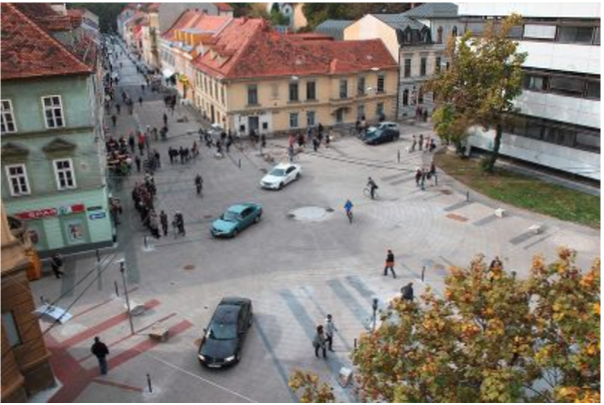
\includegraphics{figures/Billederogfigur/Perspektivering/en_andne_by.png}
  \end{adjustbox}
   \caption{Cykelsti}
    \label{fig:cykelsti}
 \end{figure}
 %(kilde:http://www.stadtentwicklung.graz.at/cms/beitrag/10136328/5030273/ 10/12-2015)
 På Sonnenfelsplatz er der ikke højdeforskel i vejen som adskiller køretøjer fra fodgængere.Trafikanterne deler og respekterer derfor hinanden om pladsen. I midten af pladsen er der lavet en lille rundkørsel.%(kilde:http://www.stadtentwicklung.graz.at/cms/beitrag/10136328/5030273/ 10/12-2015)


I indledningen er Nytorv/Østerågade beskrevet som et samlingspunkt, hvor der på tilsvarende måde færdes mange mennesker og køretøjer. I området er der mange shopping- og cafémuligheder, derudover færdes der mange mennesker i området, som transportere sig med bus og cykel. Ifølge trafiktællingerne der er foretaget i rapporten (se bilag) har Nytorv/Østerågade en års døgns trafik på 394 for biler og 3.826 for cykler på en novemberdag. I interviewet (se bilag) mener flere interviewpersoner, at bilerne og cyklisterne skaber utryghed for fodgængerne, hvilket er årsagen til, at der i rapporten fokuseres på at differentiere trafikantgrupperne. Derved at lave nogle forslag om at etablere en cykelbane i området, hvor cyklisterne kan cykle på deres egen bane, og en bussluse for at udelukke bilerne fra området, hvilket kan ses på de nedenstående billeder.
\begin{figure}[htbp]
  \centering
  \begin{adjustbox}{max width=\textwidth}
    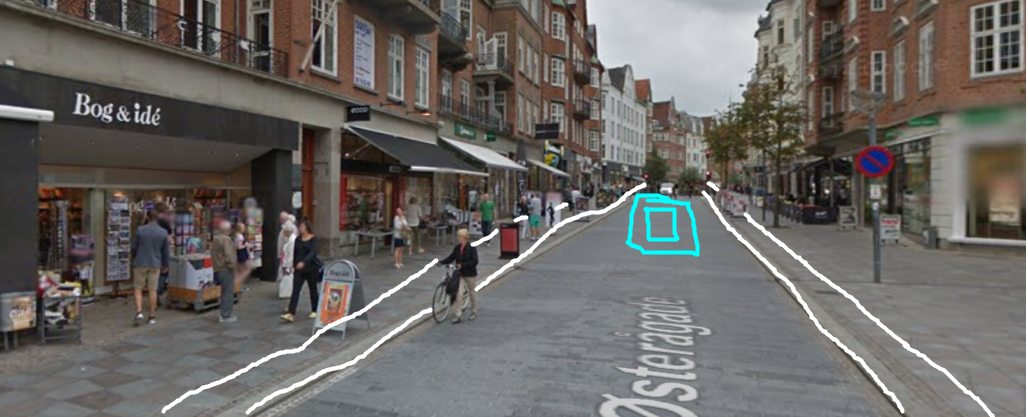
\includegraphics{figures/Billederogfigur/Losningsforslag_cykelsti/Cykelsti_gennem_bogo.png}
 \end{adjustbox}
  \caption{Cykelsti}
   \label{fig:cykelsti}
\end{figure}

\begin{figure}[htbp]
  \centering
  \begin{adjustbox}{max width=\textwidth}
    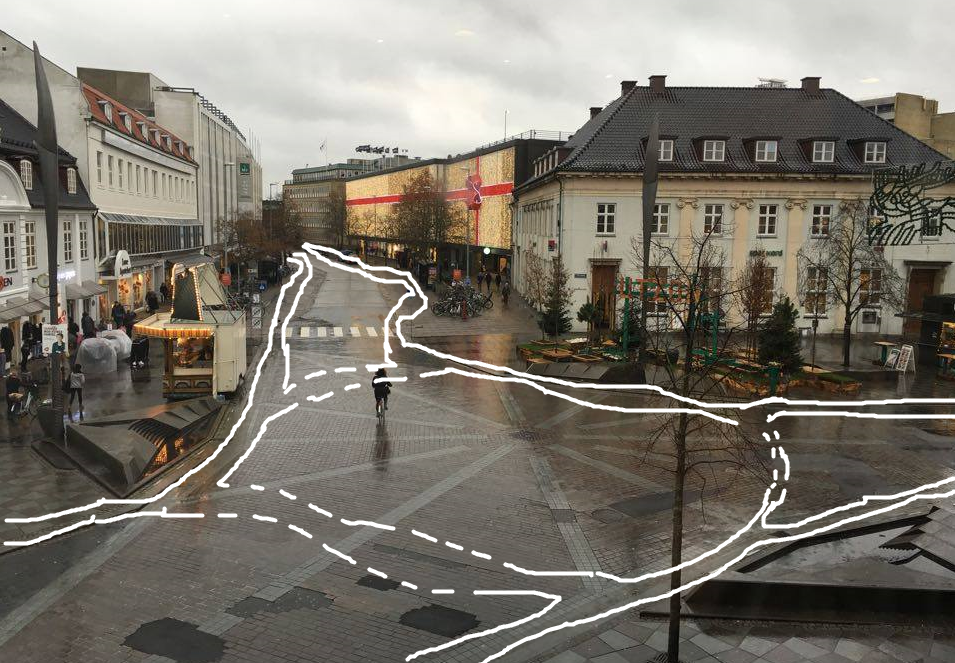
\includegraphics{figures/Billederogfigur/Losningsforslag_cykelsti/cykelsti_ved_knudepunktet.png}
 \end{adjustbox}
  \caption{Cykelsti}
   \label{fig:cykelsti}
\end{figure}
